\part{Results}
\chapter{Results}
\section{Imaging live cells}
For the study described in paper I we used cells of two species of cyanobacteria as a sample (Cyanobium gracile and Synechococcus elongatus). Cyanobacteria are photosynthetic bacteria that can be found in almost any habitat on earth, ranging from hot volcanic areas to cold polar ice caps. They play an important role in the global carbon cycle. In a 25 day cycle an algal bloom of 1000 $km^2$ can sequester around 22,000 tonnes of atmospheric carbon into organic carbon before cyanophages caused the bloom to collapse.
 
Cyanobium gracile cells were selected for their small size, their robustness with respect to the injection procedure, and convenient autofluorenscence properties to assess cell viability. Solitary C. gracile and S. elongatus cells have an oval-to-cylindrical shape, and vary in size between 0.25-0.4 $\mu$m in diameter and 0.4-4.0 $\mu$m in length [Komarek]. Cell divide symmetrically by binary fission. The two daughter cells separate from each other after reaching the size and shape of the mother cell [Komarek2]. We used non-synchronised cell cultures undergoing active growth providing cells in various stages of their cell cycle. 

The experiments described in paper I was carried out at the atomic, molecular, and optical science (AMO) endstation at LCLS at 512 eV (2.40 nm) and 1100 eV (1.13 nm) photon energy.  Figure \ref{fig:ExperimentalSetup} shows the arrangement of the experiment. The length of the photon bunch was about 70 fs. The pulse was focused to a spot of 3 $\mu m$ x 7 $\mu m$. The average photon density in the focus was about $1.1 x 10^{11}$ photons/pulse/$\mu m^2$ at 517 eV, and $8.6 x 10^{10}$ photons/pulse/$\mu m^2$ at 1,100 eV. Far-field diffraction patterns were recorded on a pair of pnCCD detectors [Struder] in the CFEL-ASG Multi Purpose (CAMP) instrument [Struder]. The detectors were place at 741 mm downstream from the interaction region of the beam and the sample. The detector read out rate matched the 120 Hz repetition rate of the LCLS. 
\begin{figure}[h]\label{fig:ExperimentalSetup}
\centering 
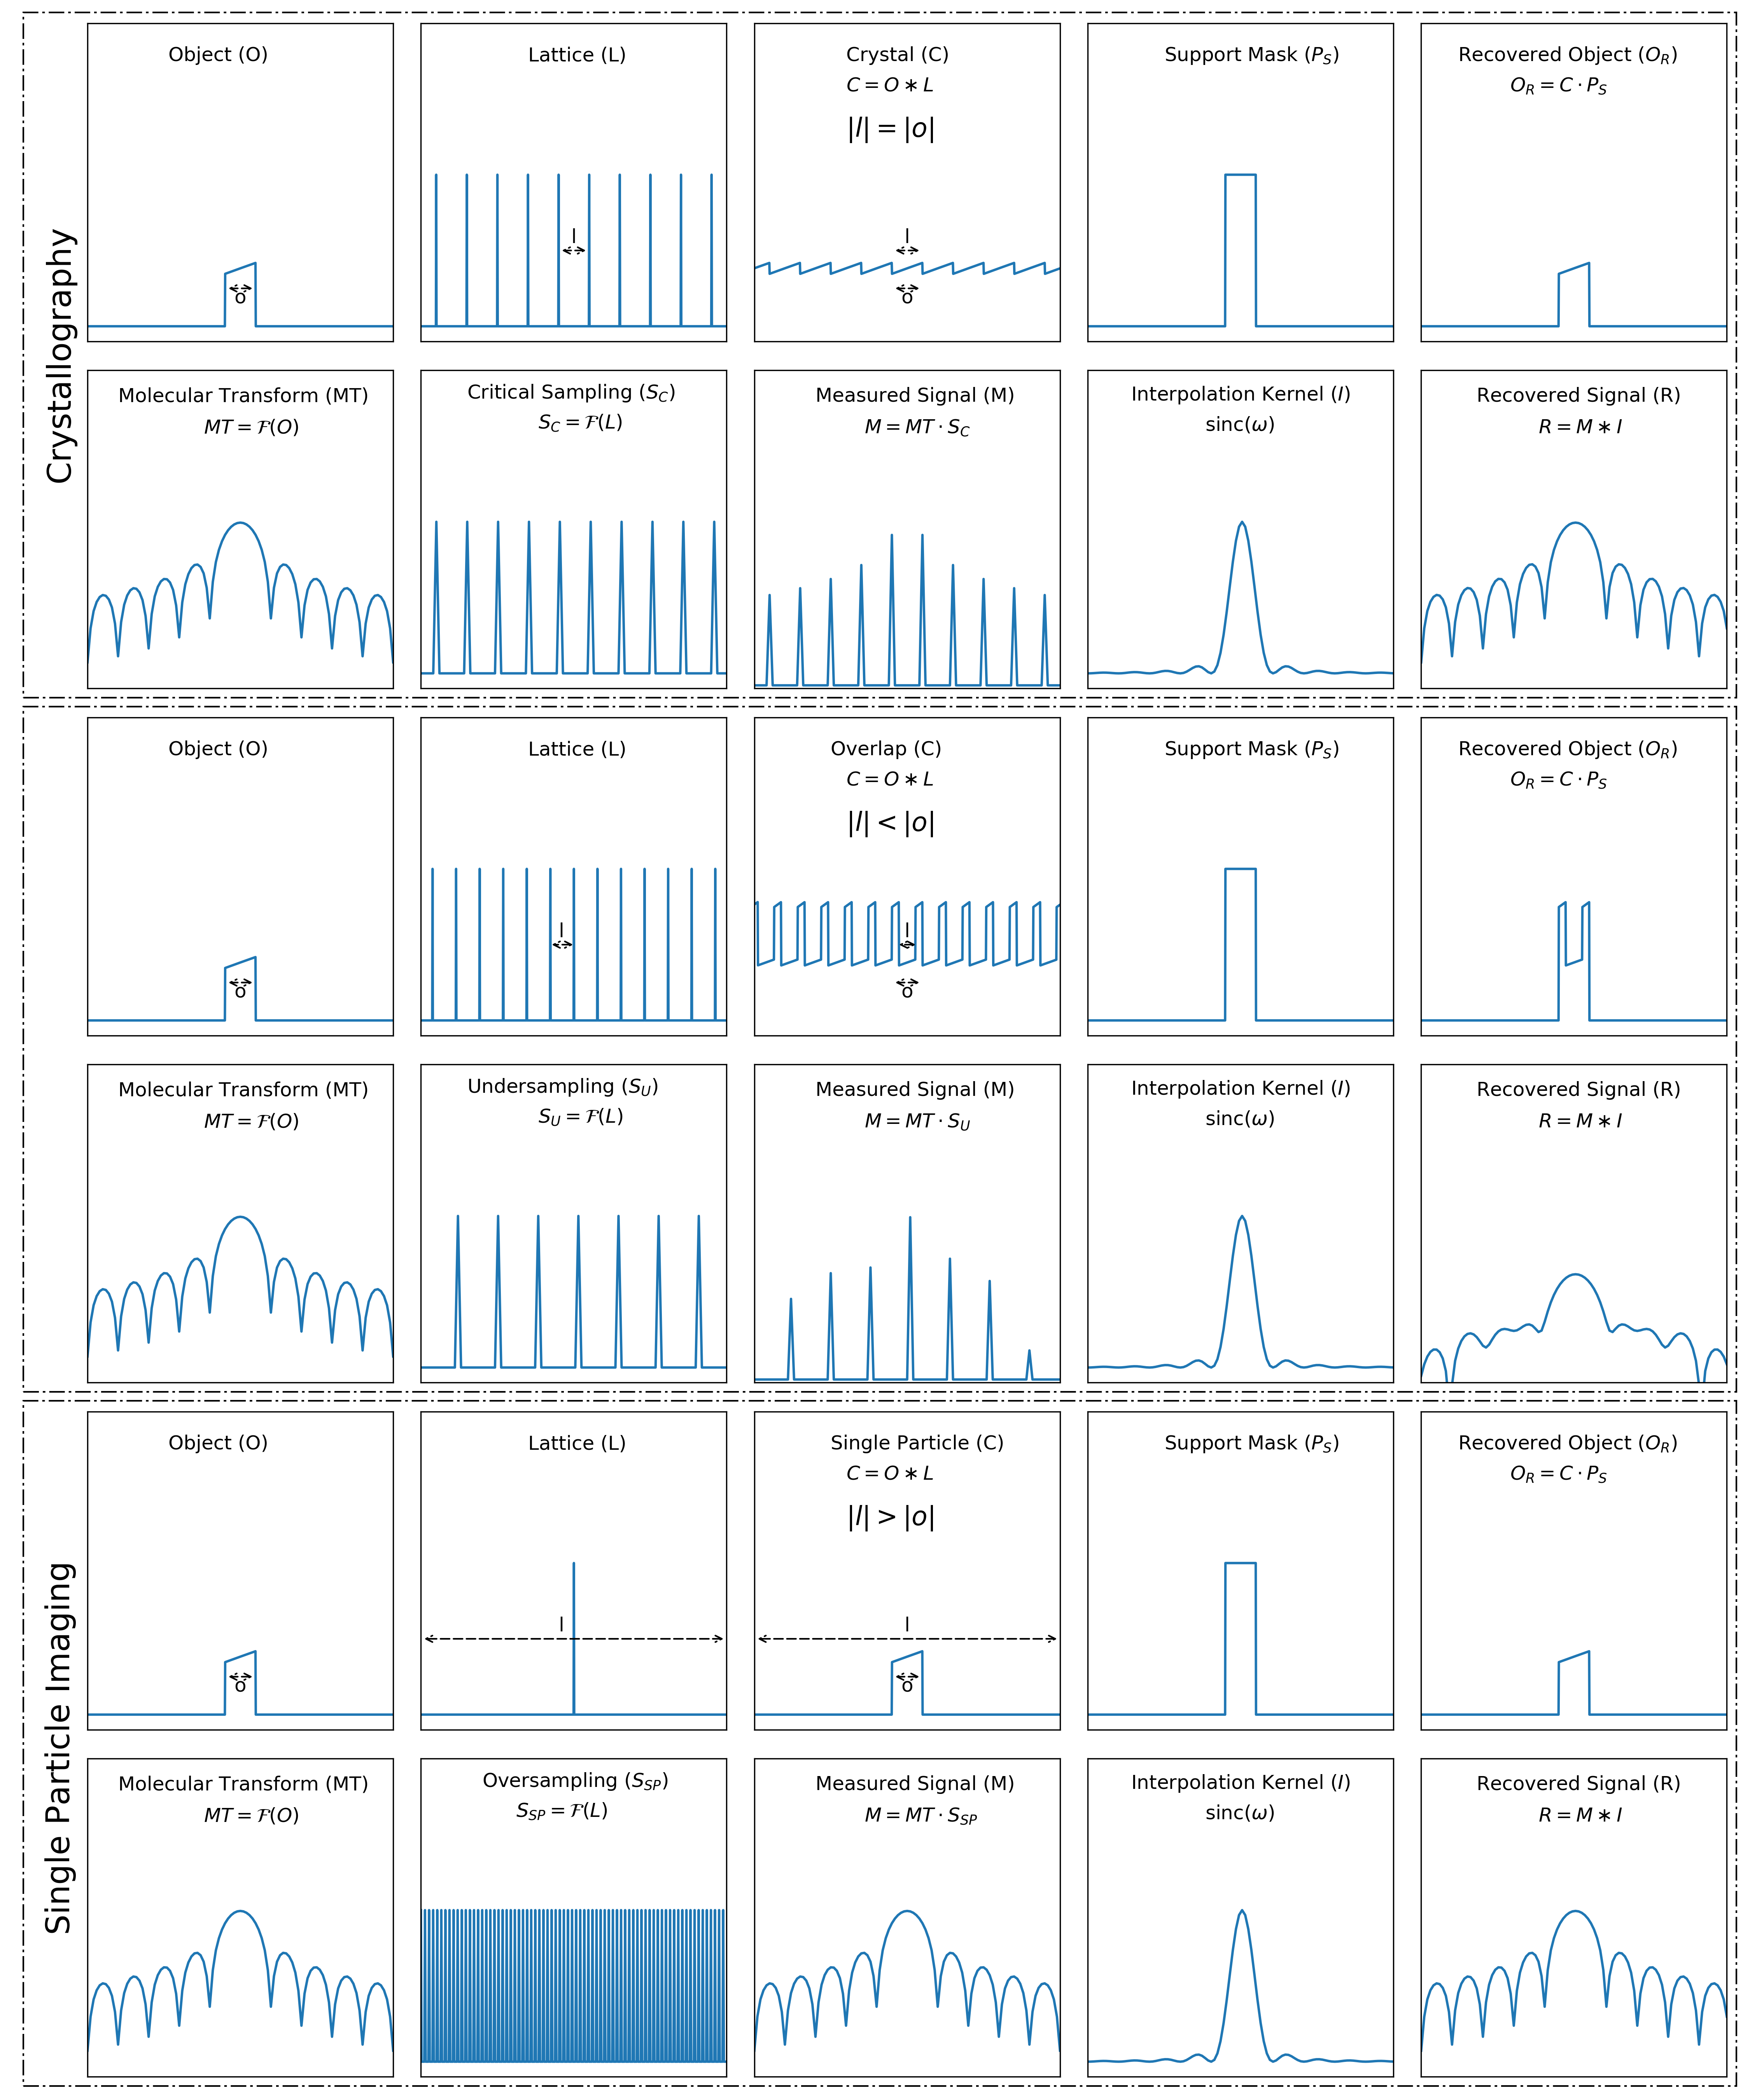
\includegraphics[width=120mm]{SamplingTheory.png}
\caption{Different rates of sampling explained}
\end{figure} 

We collected diffraction patterns of C. gracile cells for 60 minutes at a hit ratio of 43\% and selected the 7,500 clear single hits for further analysis, using the Cheetah software package. The oversampling rate of the particle was around 12-fold, which allowed direct phase recovery from the measured intensity patterns. This was not a trivial problem because strong hits saturate the detectors at low diffraction angles. As a compromise, we selected medium-strong hits, which contained either no, or only few saturated pixels while still providing scattered signal to reasonably high resolution. Missing mode analysis revealed no unconstrained modes for all cells presented in paper I. 

Figure 2 a-j shows the reconstructed exit wave-fronts (images) for ten live C. gracile cells together with the corresponding diffraction patterns, and a synthetic DIC image. The reconstructions represent 2D projections of the electron density of the cells. The images are arranged by increasing size, and show the expected morphologies of cells during division [Komarek,Komarek2]. The resolution of each  reconstruction is indicated by the size of the round white dot. Features smaller than the dot need to be interpreted with care.

Phases were retrieved using the Hawk software package. For each pattern 400 reconstructions were made, each starting from different random initial phases. These reconstructions consisted of 5000 iterations with the RAAR algorithm [Luke], using a Shrinkwrap algorithm[Machesini] for support determination, and concluded with 100 iterations by the ER algorithm[Fienup, Gerchberg-Saxton]. The initial and final support size was selected manually. No additional constraints were used since we anticipated the effects of absorption in the thick cells to give effects similar to a phase object. 

Resolution for the reconstructions was estimated from the PRTF (See Figure \ref{fig:ExperimentalSetup}), using the 1/e cutoff. Before calculating a PRTF and averaging the images we removed outliers among the reconstructions by applying a threshold to the Fourier error. Clustering validates the results from using a threshold on the Fourier-Error and the real-space error(Figures 7 a-j). On average the main cluster contained about 370 out of 400 reconstructions (93), except for one case where only 96 reconstructions formed the biggest cluster (Figure 7j). This made us believe that the average image of the main cluster is the true reconstruction minimum. Th failed reconstructions did not find the true minimum.
The scatter plots of Figure 7 a-j show that the real-space error is more reliable than the Fourier-error for identifying failed reconstructions. Furthermore, clustering aids in the identification of failed reconstructions, as it does for reconstruction 7, even if the error measures are not different. 

Detector saturation limited the achievable resolution.  In fact, the reconstructions shown in Figure \ref{fig:ExperimentalSetup} come from exposures that did not saturate the detectors. A number of much stronger exposures were also recorded, and in some of these exposures the diffraction signal extended to nanometer resolution. Figure \ref{fig:ExperimentalSetup} shows one such pattern for a live S. elongatus cell at 1,100 eV photon energy, 70 fs pulse length, about $10^11$ photons $\mu m^{-2}$ on the sample. Four pnCCD detectors were used to record this pattern (Figure \ref{fig:ExperimentalSetup}b). The configuration of the central back detector in Figure 4 is identical to the detector used in Figure 2. The front detector is the same type as the back detector but is placed at 220 mm from the interaction region. In this strong hit, a large part of the back detector was saturated, preventing reliable phasing. The signal however extended beyond 4 nm resolution on the front detectors (at sigma 3.7), which is the size of a small protein molecule. More than 58 million scattered photons were recorded on the back detectors, and 1.3 million on the front detectors. The size of the cell was derived from the autocorrelation. Figure 4c shows that in a log/log representation the drop-off of the signal is linear with spatial frequency in the range covered by our measurements, and the exponent of the signal decay is $-3.31\pm0.01$, matching simulations [Jakobson].

DICUSSION 

\section{Classification}

Sizing diffraction pattern
\\
Sizing Autocorrelation
\\
Identification multiple scatterers
\\	1) Multiple Particles
\\	2) Holographic Images
\\
Edge detection
\\
Particle shape detection
\\	1) Round particles
\\	2) Elongated Particles
\\
Success on wide variety of sizes and scattering strengths.
\\
Template-based Classification
\\

\section{Software}
